\chapter{Part 1\  循环神经网络}

\section{RNN}
\text{用于处理序列,处理序列(例如文本)的方式是,遍历序列中的所有元素,并保存一个状态,其中包含已查看内容的相关信息。}





\begin{figure}[H]
	\centering
	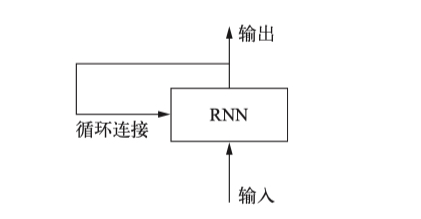
\includegraphics[width = 1.2\columnwidth]{InmemoryDatabaseExperiment/fig/2rnn1.jpg}
	\caption{RNN}
\end{figure}

\text{在处理两个不同的独立序列之间,RNN的状态都会被重置。所以仍然可以将一个序列看作单个数据点,即网络的输入。真正改变的是,数据点不再是在单个步骤中进行处理, 相反,网络内部会对序列元素进行遍历。}
\subsection{RNN的前向传递过程}

\begin{figure}[H]
	\centering
	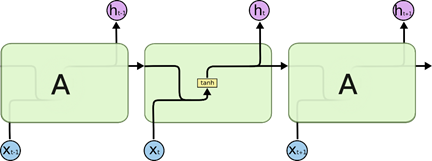
\includegraphics[width = 1.2\columnwidth]{InmemoryDatabaseExperiment/fig/rnn3.png}
	\caption{RNN前向传播}
\end{figure}
\text{如图是三个神经网络,上一个网络的信息(即ht-1)直接传过来,配合当前网络的输入Xt,两者结合之后,再通过tanh层进行信息压缩,就形成当前网络的输出ht。(这个tanh层就是一个函数,tanh就是双曲正切函数,可以将输入的值转化为-1到1之间的一个值,通常用于对信息的压缩处理,或者规范化处理。)}


\section{LSTM (长短期记忆网络)}

\text{LSTM 层是 SimpleRNN 层的一种变体,它增加了一种携带信息跨越多个时间步的方法。}
\begin{figure}[H]
	\centering
	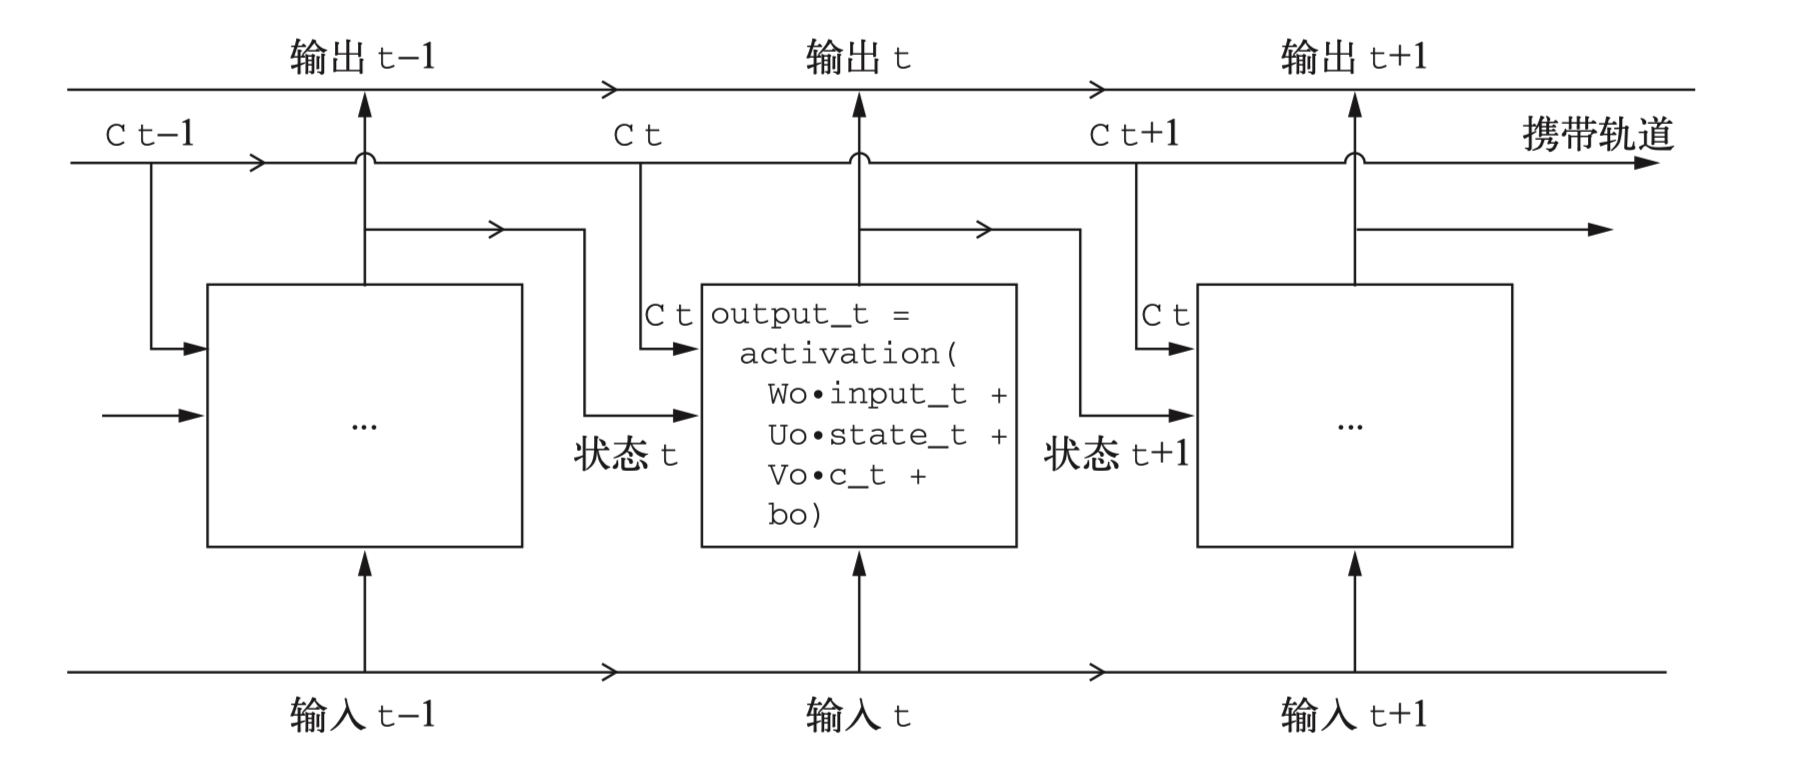
\includegraphics[width = 1.2\columnwidth]{InmemoryDatabaseExperiment/fig/lstm_2.jpg}
	\caption{LSTM}
\end{figure}

\text{我们向这张图像中添加额外的数据流,其中携带着跨越时间步的信息。它在不同的时间步 的值叫作 Ct ,其中 C 表示携带(carry)。Ct的计算方法和当前状态有关,从而会影响传递到下一个时间步的状态。}

\section{C-LSTM for text classification}


\begin{figure}[H]
	\centering
	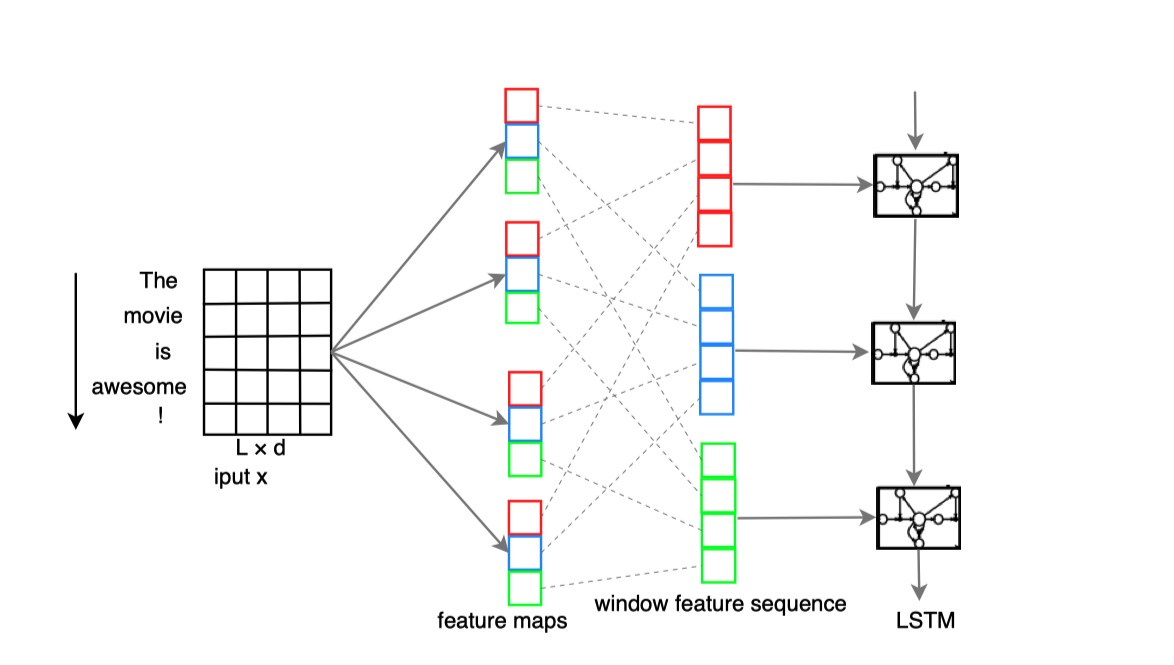
\includegraphics[width = 1.2\columnwidth]{InmemoryDatabaseExperiment/fig/clstm_2.jpg}
	\caption{C-LSTM}
\end{figure}

\subsection{一维卷积神经网络}
\text{图中的一维卷积神经网络有四个filter,每一个filter都有一个宽度为k的窗口向量,用这个窗口向量对文本序列进行划窗,本图中是划窗3次,生成一个特征图(feature map),用三种不同的颜色来代表一个filter的不同划窗的计算结果,红色,蓝色,绿色的方块代表的计算结果具有位置上的先后关系。}
\text{把所有filter的计算结果按照划窗顺序聚集在一起(相同颜色的方块放在一起),然后输入给LSTM}
\text{在LSTM的最后一步的输出后加上一softmax层,然后进行训练。}





\chapter{Part 2\  Experiment}

\section{目标}
\text{文本分类}
\section{模型}
\text{C-LSTM}
\section{数据格式(训练数据和测试数据)}
数据存储在csv文件中,分为两列,“label”列和“content”列,分别代表一条文本序列的类别和内容,总共有两类

\begin{figure}[H]
	\centering
	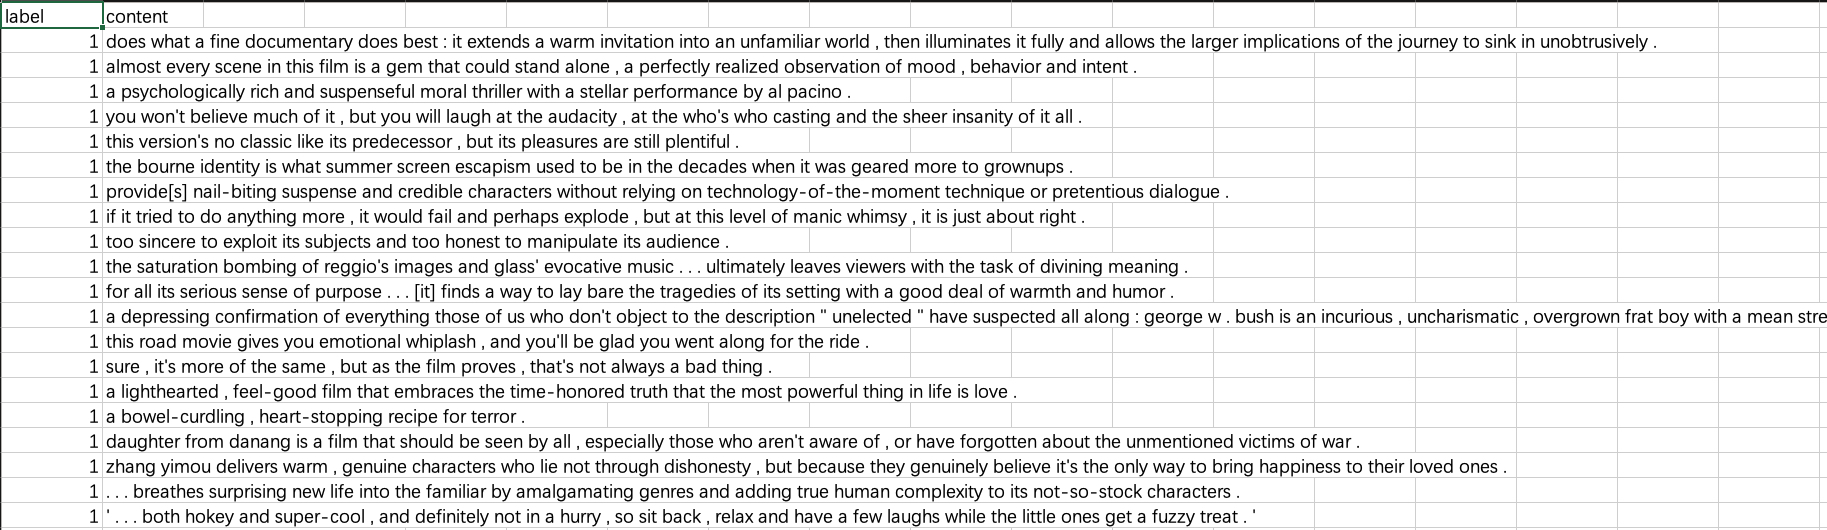
\includegraphics[width = 1.2\columnwidth]{InmemoryDatabaseExperiment/fig/data1.jpg}
	\caption{C-LSTM}
\end{figure}

\section{训练以及验证}
\begin{itemize}
    \item 使用4500条“label1”的文本和4500条“label2”的文本进行训练
    \item 在450条“label1”的文本和450条“label2”的文本上进行验证
\end{itemize}

\section{Result}

\text{在作为验证集的1000条文本中获得了76.6\%的准确率}
\begin{figure}[H]
	\centering
	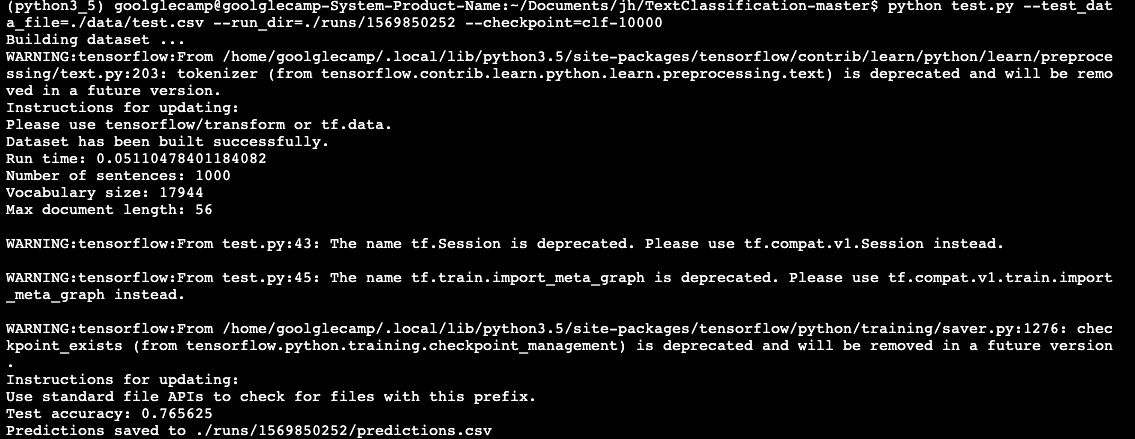
\includegraphics[width = 1.2\columnwidth]{InmemoryDatabaseExperiment/fig/predict.jpg}
	\caption{验证结果}
\end{figure}


\chapter{Part 3\  下一步工作}
\begin{itemize}
    \item 学习使用C-LSTM对异常数据序列进行分类
\end{itemize}



\chapter{Appendix A}
\listoffigures

% \chapter{Appendix B}
% \listoftables
